\chapter{実践：移動ロボットを動かす}
\label{chap:practice}

% この章で学ぶこと
\begin{goalbox}
  \begin{itemize}
    \item キーボードで移動ロボットを操作する方法
    \item LiDAR のデータを読んで、障害物を避けながら走るノードの作り方
    \item SLAM を使って、ロボットに地図を作らせる方法
    \item Navigation2 を使って、地図の上の目的地までロボットを自律移動させる方法
    \item この本の先に進むための道しるべ
  \end{itemize}
\end{goalbox}

この章では、ここまでに学んだことを総動員して、\ref{chap:simulation}章の TurtleBot3 のシミュレーションで、移動ロボットを動かしていきます。
キーボードでの操作から始めて、自分で書いたノードで障害物を避けさせ、最後は、ロボットに地図を作らせて、その地図の上で目的地まで自動で移動させます。
シミュレーションで動くようになれば、同じしくみで、実際のロボットも動かせます（\ref{chap:kachaka}章）。

この章では、すべてのノードをシミュレーションと組み合わせて使うので、自分で起動するノードには \cmd{use\_sim\_time:=true} を付けます（\ref{sec:simulation-bridge}節）。
まず、TurtleBot3 のシミュレーションを起動しておきましょう。

\begin{terminal}[TurtleBot3 のシミュレーションを起動する]
$ ros2 launch turtlebot3_gazebo turtlebot3_world.launch.py
\end{terminal}

\section{キーボードでロボットを操作する}
\label{sec:practice-teleop}

\subsection{teleop\_twist\_keyboard}

\ref{sec:simulation-turtlebot3}節では、TurtleBot3 専用の \cmd{teleop\_keyboard} でロボットを動かしました。
ROS 2 には、TurtleBot3 に限らず、どの移動ロボットでも使える \textbf{teleop\_twist\_keyboard} というノードもあります。
\cmd{/cmd\_vel} トピックに速度の指令をパブリッシュするだけなので、\cmd{/cmd\_vel} で動くロボットなら、シミュレーションでも実際のロボットでも、そのまま使えます。

\begin{terminal}[teleop\_twist\_keyboard をインストールして起動する]
$ sudo apt install ros-jazzy-teleop-twist-keyboard
$ ros2 run teleop_twist_keyboard teleop_twist_keyboard --ros-args -p stamped:=true
...
Moving around:
   u    i    o
   j    k    l
   m    ,    .
...
q/z : increase/decrease max speeds by 10%
\end{terminal}

\cmd{stamped:=true} は、\cmd{Twist} ではなく \cmd{TwistStamped}（\ref{sec:simulation-turtlebot3}節）でパブリッシュするための設定です。
ROS 2 Jazzy の TurtleBot3 は \cmd{TwistStamped} を使うので、この設定が必要です。

\key{I} で前進、\key{,} で後退、\key{J} と \key{L} でその場で回転、\key{K} で停止です。
\key{U}・\key{O}・\key{M}・\key{.} では、曲がりながら進みます。
ほかのキーを押すと停止するので、ロボットを止めたいときは、慌てずに \key{K} などを押しましょう。
はじめは速度が速すぎるので、\key{Z} を何回か押して、最大の速さを下げておくとよいでしょう。

\section{センサデータを読んで障害物を避けるノードを作る}
\label{sec:practice-avoid}

\subsection{考え方}

LiDAR のデータを読んで、障害物を避けながら走り回るノードを作ってみましょう。
ここでは、次のような簡単な方法で考えます（図\ref{fig:practice-avoid}）。

\begin{enumerate}
  \item LiDAR のデータ（\cmd{/scan}、\ref{sec:simulation-sensor}節）から、ロボットの正面（左右 30 度以内）の距離だけを取り出す
  \item その中で、最も近い距離を求める
  \item 最も近い距離が、決めておいた距離（\cmd{safe\_distance}）より近ければ、その場で左に回る。そうでなければ、まっすぐ進む
\end{enumerate}

\begin{figure}[tb]
  \centering
  % 図：LiDAR の正面の範囲で障害物を見つける（chapters/ros2/practice.tex）
\begin{tikzpicture}
  % 正面 ±30 度の範囲
  \fill[orange!15] (0,0) -- (30:3.3) arc (30:-30:3.3) -- cycle;
  \draw[orange!70!black, dashed] (0,0) -- (30:3.3) (0,0) -- (-30:3.3);
  \node[font=\scriptsize, orange!60!black, align=center] at (2.75,0.62) {正面\\（左右 30°）};
  % LiDAR の測定線
  \foreach \a in {-150,-120,...,180} {\draw[black!25] (0,0) -- (\a:2.2);}
  % ロボット
  \draw[fill=blue!10, rounded corners=2pt] (-0.35,-0.3) rectangle (0.35,0.3);
  \node[font=\scriptsize, below] at (0,-0.3) {ロボット（右が前）};
  % 障害物
  \fill[black!60] (2.1,-0.55) rectangle (2.5,0.15);
  \draw[{Stealth[length=1.8mm]}-{Stealth[length=1.8mm]}, thick, blue!70!black] (0.35,0) -- node[above, font=\scriptsize, fill=white, inner sep=1pt]{最も近い距離} (2.1,0);
  % 判定
  \node[draw, rounded corners=2pt, font=\scriptsize, align=left, anchor=west, fill=white] at (4.0,0.5) {最も近い距離 $<$ \texttt{safe\_distance}\\ \quad → その場で左に回る};
  \node[draw, rounded corners=2pt, font=\scriptsize, align=left, anchor=west, fill=white] at (4.0,-0.5) {それ以外\\ \quad → まっすぐ進む};
\end{tikzpicture}

  \caption{LiDAR の正面の範囲で障害物を見つける}
  \label{fig:practice-avoid}
\end{figure}

これは、\ref{sec:rclpy-timer}節で turtlesim のカメに壁を避けさせたのと同じ考え方です。
違うのは、カメの位置ではなく、センサで測った距離を使うところです。

\subsection{ノードのプログラム}

\cmd{my\_package} に \cmd{obstacle\_avoider.py} を作ります。

\codefile[style=python, lastline=60]{障害物を避けるノード（my\_package/obstacle\_avoider.py）}{lst:practice-avoider}{samples/rclpy/my_package/my_package/obstacle_avoider.py}

\begin{description}
  \item[パラメータ] 止まって曲がり始める距離・進む速さ・回る速さを、パラメータ（\ref{sec:rclpy-param}節）にしています。プログラムを書き換えずに、実行しながら調整できます。\cmd{front\_angle}（LiDAR から見たロボットの正面の向き）と \cmd{stamped}（\cmd{TwistStamped} で送るか、\cmd{Twist} で送るか）は、別のロボットでこのノードを使うためのパラメータで、\ref{chap:kachaka}章で使います。TurtleBot3 では初期値のままで構いません。
  \item[QoS] LiDAR のデータは \cmd{BEST\_EFFORT} でパブリッシュされることが多いので、サブスクライバの QoS に \cmd{qos\_profile\_sensor\_data} を使っています（\ref{sec:debug-qos}節）。
  \item[\cmd{scan\_callback}] \cmd{ranges} の \cmd{i} 番目の値の向きは、\cmd{angle\_min + i * angle\_increment} で計算できます。TurtleBot3 の LiDAR は、正面を 0 として 0〜$2\pi$ の範囲で測るので、\cmd{atan2} を使って $-\pi$〜$\pi$ の範囲に直し、正面からの角度を求めやすくしています。正しく測れた値（\cmd{range\_min} と \cmd{range\_max} の間）だけを使い、何も測れなかったときは、障害物がない（\cmd{math.inf}、無限に遠い）とみなします。
  \item[\cmd{timer\_callback}] 0.1 秒ごとに、最も近い距離をもとに速度の指令（\cmd{Twist}）を決めます。\cmd{stamped} が \cmd{True} なら、それを \cmd{TwistStamped} に入れてパブリッシュします。\cmd{header.stamp} には、\cmd{get\_clock().now()} で今の時刻を入れます。\cmd{use\_sim\_time} が \cmd{true} なら、シミュレーションの時刻になります。
\end{description}

\cmd{setup.py} の \cmd{entry\_points} に \cmd{'obstacle\_avoider = my\_package.obstacle\_avoider:main',} を、\cmd{package.xml} に \cmd{<depend>sensor\_msgs</depend>} を追加して、ビルドします。

\subsection{動かしてみる}

teleop\_twist\_keyboard を止めてから、障害物を避けるノードを起動します。

\begin{terminal}[障害物を避けるノードを起動する]
$ cd ~/ros2_ws
~/ros2_ws$ colcon build --symlink-install --packages-select my_package
~/ros2_ws$ source install/local_setup.bash
~/ros2_ws$ ros2 run my_package obstacle_avoider --ros-args -p use_sim_time:=true
\end{terminal}

ロボットがまっすぐ進み、柱や壁に近づくと、その場で回って向きを変え、また進んでいきます。
別のターミナルから、パラメータを変えてみましょう。

\begin{terminal}[実行中にパラメータを変える]
~/ros2_ws$ ros2 param set /obstacle_avoider safe_distance 0.8
~/ros2_ws$ ros2 param set /obstacle_avoider linear_speed 0.22
\end{terminal}

\begin{caution}[ノードを止めてもロボットは止まらない]
  \key{Ctrl}+\key{C} でノードを止めても、ロボットは最後に受け取った速度の指令のまま、動き続けることがあります。
  ロボットを止めるには、速度が 0 の指令を送ります。
\begin{lstlisting}[numbers=none, xleftmargin=0pt, framexleftmargin=0pt]
$ ros2 topic pub --once /cmd_vel geometry_msgs/msg/TwistStamped "{}"
\end{lstlisting}
  実際のロボットでは、思わぬ動きをしたときにすぐ止められるように、非常停止のボタンを用意したり、手で持ち上げられるようにしたりしておくことが大切です。
\end{caution}

\begin{point}[改良してみよう]
  このノードは、とても単純な方法で障害物を避けています。
  次のような改良を考えてみましょう。
  \begin{itemize}
    \item いつも左に回るのではなく、左右で空いているほうに回る
    \item 障害物に近づくほど、少しずつ速度を落とす
    \item 曲がっている途中も、少しずつ前に進む
  \end{itemize}
  改良したら、bag ファイル（\ref{sec:debug-rosbag}節）に \cmd{/scan} と \cmd{/cmd\_vel} を記録して、動きを比べてみるのもよいでしょう。
\end{point}

\section{SLAM による地図作成の体験}
\label{sec:practice-slam}

\subsection{SLAM とは}

ロボットが部屋の中を目的地まで移動するには、部屋の地図と、その地図の上で自分がどこにいるかが必要です。
しかし、地図を作るには自分の位置が必要で、自分の位置を知るには地図が必要、という「卵が先か、鶏が先か」のような問題があります。
そこで、ロボットを動かしながら、センサのデータから、地図作りと自分の位置の推定を同時に行います。
これを \textbf{SLAM}（Simultaneous Localization and Mapping）といいます。

ROS 2 では、LiDAR を使った SLAM のパッケージとして、\textbf{slam\_toolbox} がよく使われます。
slam\_toolbox は、\cmd{/scan} と、オドメトリの座標変換（\cmd{odom} → \cmd{base\_link}）を使って地図を作り、\cmd{/map} トピックにパブリッシュします。
また、オドメトリのずれを補正する \cmd{map} → \cmd{odom} の座標変換も、tf2 に流します（\ref{sec:tf-viz-frames}節）。

\subsection{地図を作る}

slam\_toolbox をインストールして、起動します。
シミュレーションは起動したままにしておきます（障害物を避けるノードは止めておきます）。

\begin{terminal}[slam\_toolbox をインストールして起動する]
~/ros2_ws$ sudo apt install ros-jazzy-slam-toolbox
~/ros2_ws$ ros2 launch slam_toolbox online_async_launch.py use_sim_time:=true
\end{terminal}

作っている地図を見るために、RViz2 を起動して、次のように設定します（\ref{sec:tf-viz-rviz}節）。

\begin{terminal}[RViz2 を起動する]
~/ros2_ws$ rviz2 --ros-args -p use_sim_time:=true
\end{terminal}

\begin{enumerate}
  \item 「Fixed Frame」を \cmd{map} にします。
  \item 「Add」の「By topic」タブから、\cmd{/map} の「Map」と、\cmd{/scan} の「LaserScan」を追加します。
  \item 「Add」から「RobotModel」を追加し、「Description Topic」を \cmd{/robot\_description} にします。
\end{enumerate}

teleop\_twist\_keyboard でロボットをゆっくり動かして、世界の中をひととおり走らせてみましょう。
ロボットが動くにつれて、地図が少しずつできていきます（図\ref{fig:practice-slam}）。
地図の白いところは通れる場所、黒いところは障害物、灰色のところはまだわからない場所です。
このような地図を\textbf{占有格子地図}（Occupancy Grid Map）といいます。

\begin{figure}[tb]
  \centering
  \large
  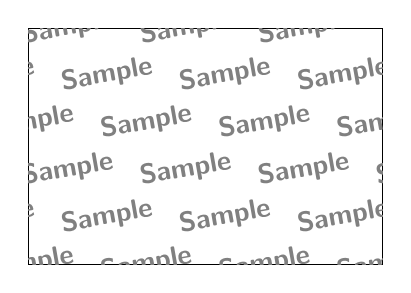
\begin{tikzpicture}
    \draw rectangle++(4.5,3);
    \clip rectangle++(4.5,3);
    \foreach\x in{0,1,2,3,4}{
      \foreach\y in{0,1,2,3,4,5,6}{
        \path(\x*1.5-\y*0.5,\y*0.6)node[rotate=10,text=gray]{\sffamily\bfseries\itshape Sample };
      }
    }
  \end{tikzpicture}
  %% 入れる画像：slam_toolbox で turtlebot3_world の地図を作っている途中の RViz2 の画面（Map・LaserScan・RobotModel を表示）のスクリーンショット
  % eps 画像を貼る場合は includegraphics をお使いください。
  % \includegraphics[width=0.8\linewidth]{practice/slam.png}
  \caption{SLAM で地図を作っている様子}
  \label{fig:practice-slam}
\end{figure}

\begin{point}[きれいな地図を作るコツ]
  \begin{itemize}
    \item ゆっくり動かす。特に、その場での回転は、ゆっくり行う
    \item 同じ場所を何度か通り、ぐるりと 1 周して出発した場所に戻ってくる（ループを閉じる）と、ずれが補正されて地図がきれいになる
    \item 障害物が少なく、特徴のない長い廊下などでは、地図がずれやすい
  \end{itemize}
\end{point}

\subsection{地図を保存する}

地図ができたら、ファイルに保存します。
Navigation2 の \cmd{map\_saver\_cli} を使います。

\begin{terminal}[地図を保存する]
~/ros2_ws$ sudo apt install ros-jazzy-navigation2 ros-jazzy-nav2-bringup
~/ros2_ws$ ros2 run nav2_map_server map_saver_cli -f ~/map --ros-args -p use_sim_time:=true
...
[INFO] [...] [map_saver]: Map saved successfully
~/ros2_ws$ ls ~/map.*
/home/user/map.pgm  /home/user/map.yaml
\end{terminal}

\cmd{map.pgm} は地図の画像、\cmd{map.yaml} は地図の大きさ（1 ピクセルが何メートルか）や原点の位置などを書いた設定ファイルです。
次の節で、この地図を使います。
保存したら、slam\_toolbox と RViz2 は止めておきましょう。

\section{Navigation2 による自律移動の体験}
\label{sec:practice-nav2}

\subsection{Navigation2 とは}

\textbf{Navigation2}（Nav2）は、移動ロボットを、地図の上の目的地まで自動で移動させるためのパッケージの集まりです。
目的地を指示すると、次のようなことを行ってくれます。

\begin{description}
  \item[自己位置推定] 保存した地図と LiDAR のデータを照らし合わせて、地図の上でのロボットの位置を推定します（AMCL というしくみを使います）。
  \item[経路計画] 地図の上で、今の位置から目的地までの経路を計画します。
  \item[経路追従と障害物回避] 計画した経路に沿って進むように、速度の指令を出します。地図にない障害物（人や箱など）が現れたら、それを避けます。
  \item[リカバリ] 行き詰まったときに、少し下がったり回ったりして、抜け出そうとします。
\end{description}

\subsection{自律移動させる}

TurtleBot3 には、Navigation2 を TurtleBot3 用の設定で起動する launch ファイルが用意されています。
シミュレーションを起動したまま、前の節で保存した地図を指定して起動します。

\begin{terminal}[Navigation2 を起動する]
~/ros2_ws$ ros2 launch turtlebot3_navigation2 navigation2.launch.py use_sim_time:=True map:=$HOME/map.yaml
\end{terminal}

Navigation2 の設定が済んだ RViz2 が、一緒に起動します。
次の手順で、ロボットを動かしてみましょう。

\begin{enumerate}
  \item \textbf{初期位置を教える}：RViz2 の上のツールバーの「2D Pose Estimate」を押し、地図の上でロボットがいる位置をクリックして、そのままロボットが向いている方向にドラッグします。LiDAR の点が地図の壁や柱と重なれば、うまく位置を教えられています。
  \item \textbf{目的地を指示する}：ツールバーの「Nav2 Goal」を押し、地図の上の行きたい場所をクリックして、着いたときに向いていてほしい方向にドラッグします。
\end{enumerate}

ロボットが経路を計画し、柱を避けながら、目的地まで自動で移動します（図\ref{fig:practice-nav2}）。
RViz2 には、計画した経路や、障害物の周りの「近づかないほうがよい範囲」（\textbf{コストマップ}）が色付きで表示されます。

\begin{figure}[tb]
  \centering
  \large
  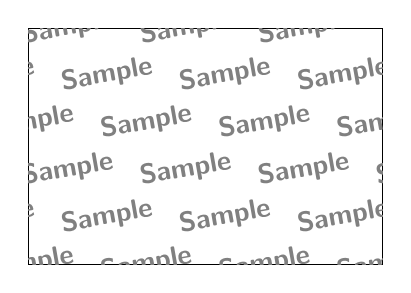
\begin{tikzpicture}
    \draw rectangle++(4.5,3);
    \clip rectangle++(4.5,3);
    \foreach\x in{0,1,2,3,4}{
      \foreach\y in{0,1,2,3,4,5,6}{
        \path(\x*1.5-\y*0.5,\y*0.6)node[rotate=10,text=gray]{\sffamily\bfseries\itshape Sample };
      }
    }
  \end{tikzpicture}
  %% 入れる画像：turtlebot3_navigation2 の RViz2 で、Nav2 Goal を指示し、計画された経路とコストマップが表示されている画面のスクリーンショット
  % eps 画像を貼る場合は includegraphics をお使いください。
  % \includegraphics[width=0.8\linewidth]{practice/nav2.png}
  \caption{Navigation2 で目的地まで自律移動している様子}
  \label{fig:practice-nav2}
\end{figure}

\subsection{目的地はアクションで指示する}

「Nav2 Goal」で目的地を指示したとき、裏では、\ref{sec:ros2-concepts-action}節で学んだ\textbf{アクション}が使われています。
目的地までの移動は時間がかかり、途中経過（残りの距離など）を知りたく、途中でキャンセルもしたいので、アクションがぴったりなのです。
アクションの一覧を見てみましょう。

\begin{terminal}[Navigation2 のアクションを調べる]
~/ros2_ws$ ros2 action list
...
/navigate_to_pose
...
\end{terminal}

\cmd{/navigate\_to\_pose} が、目的地まで移動させるアクションです。
コマンドから、ゴールを送ってみましょう。
\cmd{orientation} の \cmd{w: 1.0} は、地図の x 軸の方向（ヨーが 0）を向くという意味です（クォータニオン、\ref{sec:tf-viz-tf2}節）。

\begin{terminal}[コマンドから目的地を指示する]
~/ros2_ws$ ros2 action send_goal /navigate_to_pose nav2_msgs/action/NavigateToPose "{pose: {header: {frame_id: map}, pose: {position: {x: 1.0, y: 0.5}, orientation: {w: 1.0}}}}" --feedback
\end{terminal}

ロボットが地図の (1.0, 0.5) の位置に向かって移動し、途中経過として、残りの距離などがフィードバックで表示されます。
つまり、\ref{sec:rclpy-action}節で書いたアクションクライアントと同じようにノードを書けば、自分のプログラムからロボットを好きな場所に移動させられる、ということです。
Python から Navigation2 を使うための、\cmd{nav2\_simple\_commander} という便利なライブラリも用意されています。

\section{次のステップへ}
\label{sec:practice-next}

この本で学んだことを使えば、ロボットのソフトウェア開発の基本的な流れは、ひととおり体験できたことになります。
最後に、この先に進むための道しるべを紹介します。

\subsection{実際のロボットを動かす}

この章では、シミュレーションで TurtleBot3 を動かしました。
次の\ref{chap:kachaka}章では、家庭用ロボットのカチャカを使って、実際のロボットを動かします。
TurtleBot3 の実機では、ロボットに載っているコンピュータ（Raspberry Pi）で、モータと LiDAR を動かすノードを起動し、パソコンとはネットワーク（\ref{sec:ros2-install-network}節）でつながります。
あとは、この章とほぼ同じコマンドで、地図を作り、自律移動させられます。
実際のロボットでは、シミュレーションにはなかった問題（センサの雑音、車輪のすべり、ネットワークの遅れ、バッテリ切れ……）にたくさん出会うはずです。
それらに一つ一つ向き合うことが、ロボット開発のいちばん面白いところでもあります。

\subsection{さらに学ぶ}

興味に合わせて、次のようなテーマに進んでみましょう。

\begin{description}
  \item[ロボットアーム] ROS 2 でアームを動かすには、動作計画のフレームワーク \textbf{MoveIt 2} がよく使われます。
  \item[画像処理と認識] カメラの画像を OpenCV で処理したり、深層学習で物体を認識したりして、その結果を ROS 2 のノードで使います。
  \item[C++] 速さが求められるノードを書くために、C++ と rclcpp を学びましょう（補章\ref{sup:rclcpp}）。
  \item[マイコン] \textbf{micro-ROS} を使うと、マイコン（\ref{chap:computer}章）の上でも ROS 2 のノードを動かせます。
  \item[ロボットの理論] 座標変換、自己位置推定、経路計画、制御などの理論を学ぶと、パッケージが中で何をしているのかがわかり、自分で改良できるようになります。
\end{description}

\subsection{コミュニティに参加する}

ROS 2 は、世界中の人が開発しているオープンソースソフトウェアです（\ref{sec:linux-oss}節）。
ROS 2 の公式のドキュメントや、質問のためのフォーラムなど、学ぶための場所がたくさんあります（付録\ref{app:references}）。
わからないことを質問するときは、何をしたのか、何が起きたのか、エラーメッセージ、使っている環境（Ubuntu と ROS 2 のバージョン）を、ほかの人が再現できるように書きましょう。

慣れてきたら、使っているパッケージの不具合を Issue で報告したり、ドキュメントの誤りを直す Pull Request を送ったりしてみましょう（\ref{sec:git-github}節）。
小さな貢献でも、世界中のロボット開発者の役に立ちます。
ロボットの大会（競技会）に参加して、仲間と一緒にロボットを作るのも、力を伸ばすよい機会です。

この本が、あなたがロボットを動かすための、最初の一歩になれば幸いです。

\section*{この章のまとめ}

\begin{itemize}
  \item teleop\_twist\_keyboard を使うと、\cmd{/cmd\_vel} で動くどんな移動ロボットも、キーボードで操作できます。
  \item LiDAR のデータ（\cmd{/scan}）を読んで速度の指令（\cmd{/cmd\_vel}）を出すノードで、障害物を避けながら走らせられます。
  \item SLAM（slam\_toolbox）で、ロボットを動かしながら地図を作り、\cmd{map\_saver\_cli} で保存できます。
  \item Navigation2 は、地図の上での自己位置推定・経路計画・障害物回避を行い、ロボットを目的地まで自律移動させます。目的地はアクションで指示します。
  \item 実際のロボット、さらに進んだテーマ、コミュニティへの参加へと、次のステップに進みましょう。
\end{itemize}
